\documentclass[graybox]{svmult}

% Springer fonts and formatting
\usepackage{mathptmx}       % selects Times Roman as basic font
\usepackage{helvet}         % selects Helvetica as sans-serif font
\usepackage{courier}        % selects Courier as typewriter font
\usepackage{type1cm}        % activate if fonts are not available on system

\usepackage{makeidx}         % allows index generation
\usepackage{graphicx}        % standard LaTeX graphics tool
\usepackage{multicol}        % used for the two-column index
\usepackage[bottom]{footmisc}% places footnotes at page bottom

\usepackage{amsmath,amssymb,amsfonts}
\usepackage{booktabs}
\usepackage[hidelinks]{hyperref}
\usepackage{microtype}
\usepackage{xcolor}

% Custom macros and notations
% Macros inlined
% Reliance-Utility Benchmark Macros and Math Notation

% Number verification macro: \checknum{value}{model:corruption:column}
% Expands to the value in LaTeX, and is verified by scripts/check_numbers.py
\newcommand{\checknum}[2]{#1}

% Placeholder macro for pending empirical results
\newcommand{\TODO}[1]{\textcolor{red}{[\textbf{TODO}: #1]}}

% Common notation macros
\newcommand{\utility}{U(S)}
\newcommand{\reliance}{R(S)}
\newcommand{\normreliance}{\hat{R}(S)}
\newcommand{\crossing}{S^*}
\newcommand{\mi}{\text{MI}}
\newcommand{\jsd}{\text{JSD}}
\newcommand{\dkl}{D_{\text{KL}}}

% Abstract keywords macro (used in svmult \keywords{} call)
\providecommand{\keywords}[1]{\par\addvspace{0.5\baselineskip}\noindent\textbf{Keywords:} #1}

% Compress paragraph heading spacing to run-in style
\makeatletter
\renewcommand\paragraph{\@startsection{paragraph}{4}{\z@}%
  {-6\p@ \@plus -2\p@ \@minus -2\p@}%
  {-0.5em}%
  {\normalfont\normalsize\bfseries}}
\makeatother


\makeindex             % used for the subject index

\begin{document}
\raggedbottom

\title*{Reliance-Utility Misalignment in Multimodal AI: Formal Framework and Multi-Model Evaluation}
\titlerunning{Reliance-Utility Misalignment in Multimodal AI}

\newif\ifanon
\anontrue   % anonymous PDF for review; set \anonfalse for a named version

\ifanon
  \author{Anonymous Authors}
  \authorrunning{Anonymous Authors}
  \institute{Anonymous Authors \at Anonymous Institution, Anonymous Address}
\else
  \author{Mohammed Farhan Siddiqui and Uma Rani}
  \authorrunning{M. F. Siddiqui and U. Rani}
  \institute{Mohammed Farhan Siddiqui \at Department of Computer Science, ADGIPS,
  New Delhi, India, \\ \email{MohammedFarhan678@outlook.com}
  \and Uma Rani (corresponding author) \at Department of Computer Science,
  ADGIPS, New Delhi, India, \\ \email{dr.uma@adgips.ac.in}}
\fi

\maketitle

% Inlined from sections/abstract.tex
\abstract{%
In this paper we evaluate multimodal models. Multimodal models are usually
evaluated by assigning them a task and then investigating whether
performance drops when one input is degraded. This mixes up two different
things: information that is lost due to degradation, and a model that still
keeps relying on an input after it has stopped helping. We propose a
black-box diagnostic that separates the two. Along a severity path we pair
utility with reliance and locate where utility falls below the no-input
level. We evaluate our measures on synthetic fusion models implemented with
controlled reliance, including an oracle control. On three open VLMs and a
multiple-choice VQA task, a swapped-image corruption leaves normalized
reliance at \checknum{0.487}{Qwen:swapblend:R_hat_s1} to
\checknum{0.578}{llava:swapblend:R_hat_s1} of its clean level,
\checknum{0.112}{paired:SmolVLM:delta_rhat} to
\checknum{0.319}{paired:Qwen:delta_rhat} above Gaussian noise,
and produces a significant utility inversion for one model under both
baselines. The pre-declared criterion was met in only
\checknum{2}{criterion:status:count_met} of the 42 combinations, and
conclusions for individual models depend on how the no-input baseline was
defined. A small modality-dropout study preserves clean accuracy but shows a
clear drop in raw reliance, while exposing a weakness of R(0)-normalized
measures.}
\keywords{Multimodal Learning, Vision-Language Models, Robustness Evaluation, Intelligent Systems}

% Inlined from sections/intro.tex
\section{Introduction}
\label{sec:intro}

When one input to a multimodal system degrades, the usual evaluation asks
whether task performance falls. A drop has at least two causes. The
information needed for the task may have been destroyed. Or the information
may remain available in another input while the model keeps relying on the
degraded one. Accuracy alone does not distinguish these cases.

Substituting or removing an input to probe a model's dependence on it is
established practice (Sect.~\ref{sec:related}). What we study is a
severity-graded version: how performance and reliance change together as
one input is degraded step by step. For each severity we measure
\emph{utility}, the task performance with the degraded input relative to
removing it, and \emph{reliance}, the divergence between the model's
answer distributions with the degraded and with the removed input. We
locate where utility first reaches zero and ask how much reliance remains
there. To our knowledge, this pairing along a severity path has not been
studied in the work we reviewed.

\paragraph{Contributions.}
(i) We define the diagnostic: utility, reliance, a normalized reliance
$\hat R$, a utility-crossing severity, and a Misalignment Index (MI)
summarizing reliance beyond the crossing. (ii) We evaluate it on synthetic
fusion models with controlled reliance, including an oracle control. Our
first pre-set success criterion failed, and the revised criterion is
reported as post hoc. (iii) We apply it to three open VLMs on
multiple-choice VQA, with a held-out replication and an analysis of how
conclusions depend on the no-input baseline. (iv) We evaluate a pre-declared criterion (a criterion recorded with a timestamp in a version-controlled log before the experiments) that is met in only \checknum{2}{criterion:status:count_met} of 42
combinations. (v) We
include a small modality-dropout proxy study.

% Inlined from sections/related.tex
\section{Related Work}
\label{sec:related}

\paragraph{Modality interference.}
Cai et al.~\cite{cai2025interference} study how signals from a
non-essential modality distort multimodal LLM decisions by applying discrete
perturbations to an irrelevant input and measuring argmax answer changes.
We instead degrade the informative modality along a continuous severity path
and relate the resulting distributional behaviour change to task utility.

\paragraph{Counterfactual grounding probes.}
Substituting blank or mismatched images to test visual dependence is
established practice. Zafar et al.~\cite{zafar2026grounding} compare real,
blank and shuffled images in medical VQA and report a visual reliance
score (accuracy with the real image minus accuracy with a shuffled one),
a blank-image accuracy drop, and an answer-change rate under shuffling;
they note that accuracy-based and answer-level metrics can disagree. Work
on over-reliance on visual context in VQA~\cite{gupta2022swapmix}
and on language priors in VLMs~\cite{goyal2017making,agrawal2018dont} is
closely related. Our swapped
condition at maximum severity is comparable to a shuffled-image probe. The
difference is that we trace a trajectory over severity, measure reliance
as divergence between full answer distributions rather than answer
changes, and locate the severity at which utility falls below the
no-image level.
OMD-Bench~\cite{nazi2026omd} replaces whole modality channels in
initially congruent video, audio and text inputs and evaluates
accuracy, calibrated abstention and confidence. It defines reliance as the
fractional accuracy drop when a modality is corrupted, and its authors
note that its binary corruption model may not transfer to graded
degradation. Our severity path addresses that regime directly, although
we restrict ourselves to one visual modality and a multiple-choice
format.

\paragraph{Quality-aware fusion.}
Moon et al.~\cite{moon2026quality} use positive controls to test whether
quality scores in fusion models influence decisions, separating outage from
degradation. We borrow the positive-control strategy in our synthetic
validation, but evaluate reliance directly on the degraded input rather than on
an auxiliary quality score.

\paragraph{Missing modalities and modality dropout.}
Robustness to absent modalities has been studied extensively
\cite{ma2022missing}; modality dropout as a training
technique~\cite{neverova2016moddrop} forces networks to learn robust
cross-modal features.
Our fusion study in Sect.~\ref{sec:fusion} trains small two-view models
with different modality-dropout rates and reports clean accuracy,
no-input accuracy and reliance; it is a proxy study and not a claim about
large multimodal systems.

% Inlined from sections/method.tex
\section{Methodology: Measuring Reliance-Utility Misalignment}
\label{sec:method}

\subsection{Formal Formulation and Notation}
Let $X = (X_m, X_{\text{rest}})$ denote a multimodal input instance, where $X_m$ is the target modality under study (e.g., visual input in Vision-Language Models) and $X_{\text{rest}}$ denotes the remaining contextual modalities (e.g., text prompt and instructions). We evaluate the model's behavior under a calibrated family of corruption operators $T_m(X_m, S)$, parameterized by degradation severity $S \in [0, 1]$, where $S=0$ represents clean, uncorrupted input and $S=1$ corresponds to complete informational degradation.

Let $f(\cdot)$ denote a multimodal predictive model producing output distribution $B$. The predictive distribution under severity $S$ is:
\begin{equation}
B_m(S) = f(T_m(X_m, S), X_{\text{rest}})
\end{equation}
We define the unimodal null baseline behavior as:
\begin{equation}
B_{\text{null}} = f(\text{null}_m, X_{\text{rest}})
\end{equation}
where $\text{null}_m$ represents the complete absence or neutralization of modality $m$. In our primary benchmarks, the canonical null is the \emph{removed} condition, where visual tokens are completely omitted from the model sequence, alongside the \emph{black} image baseline (all-zero image).

\paragraph{Corruptions.}
Two primary corruption operators are studied: (i)~\emph{Swapblend}: at severity $S$, the input image is blended as $(1-S)\cdot\text{img} + S\cdot\text{img}_{\text{other}}$, where $\text{img}_{\text{other}}$ is the image of another question selected by a fixed derangement (resized bilinearly to match), with complete image substitution at $S=1$; (ii)~\emph{Gaussian blend}: $(1-S)\cdot\text{img} + S\cdot\text{noise}$, where noise is drawn from $\mathcal{N}(128, \sigma_{\text{img}})$ and clipped to $[0, 255]$.

\subsection{Multimodal Utility $U(S)$}
Multimodal utility measures the task performance benefit gained by providing the degraded modality $X_m$ at severity $S$ relative to the unimodal null baseline:
\begin{equation}
U(S) = \text{acc}(B_m(S)) - \text{acc}(B_{\text{null}})
\end{equation}
where $\text{acc}(\cdot)$ denotes classification accuracy on the target evaluation set.
When $U(S) > 0$, the degraded modality provides net positive value. When $U(S) \le 0$, the modality has become useless or actively harmful compared to ignoring it altogether.

\subsection{Information-Theoretic Reliance $R(S)$ and Normalized Reliance $\hat{R}(S)$}
Behavioral reliance quantifies the extent to which the model's output distribution shifts when conditioned on the corrupted modality versus the null baseline. We operationalize reliance via the Jensen-Shannon Divergence ($\jsd$)~\cite{lin1991divergence} in base-2 logarithm:
\begin{equation}
R(S) = \mathbb{E}_x \left[ \jsd(B_m(S) \parallel B_{\text{null}}) \right]
\end{equation}
where $\jsd(P \parallel Q) = \frac{1}{2} \dkl\left(P \parallel \frac{P+Q}{2}\right) + \frac{1}{2} \dkl\left(Q \parallel \frac{P+Q}{2}\right)$, strictly bounded in $[0, 1]$.

To enable meaningful cross-model and cross-architecture comparisons, we define normalized reliance relative to the clean baseline:
\begin{equation}
\hat{R}(S) = \frac{R(S)}{R(0)}
\end{equation}
where $R(0) > 0$ represents clean behavioral reliance. When $\hat{R}(S) \approx 1$, the model maintains its original reliance despite degradation. When $\hat{R}(S) \to 0$, the model discounts the degraded modality.

\subsection{Utility Crossing Point $S^*$}
The utility crossing point $S^*$ marks the severity threshold where the degraded modality ceases to deliver positive task utility:
\begin{equation}
S^* = \min \left\{ S \in [0, 1] \mid U_{\text{smooth}}(S) \le 0 \right\}
\end{equation}
where $U_{\text{smooth}}(S)$ is computed with a 3-point moving average. If $U_{\text{smooth}}(S) > 0$ across all grid points, $S^* = \text{None}$. If $S^*$ occurs at the final grid point ($S=1$), the crossing interval $[S^*, 1]$ is degenerate and reported as an edge case with no usable integration interval.

Additionally, to account for sampling variance, we evaluate the \emph{significant crossing point}, defined as the first severity level $S$ where the upper bound of the 95\% bootstrap confidence interval of $U(S)$ falls strictly below zero.

\subsection{Misalignment Index ($\mi$)}
The Misalignment Index quantifies cumulative unwarranted reliance exhibited by the model over the negative-utility regime $[S^*, 1]$:
\begin{equation}
\mi = \frac{1}{1 - S^*} \int_{S^*}^1 \hat{R}(S) \, dS
\end{equation}
computed via the trapezoid integration rule. When $S^* = \text{None}$, $\mi = \text{None}$.
Unlike earlier formulations, $\mi$ is intentionally left unclipped at the upper boundary: if severe degradation actively causes the model's predictive divergence to exceed its clean baseline ($\hat{R}(S) > 1$), $\mi$ exceeds 1.0, reflecting reliance above its clean level.

\subsection{Bootstrap Inference and Confidence Intervals}
We use $B=1000$ percentile bootstrap resamples over questions (fixed seed 42) throughout; all reported intervals are 95\% bootstrap CIs. For the synthetic study a two-level hierarchical resample additionally varies random seeds to capture across-run initialization variability alongside within-run item variability.

% Inlined from sections/synthetic.tex
\section{Validation on Synthetic Benchmark}
\label{sec:synthetic}

To examine the measures where the answer is known before evaluating large-scale models, we implemented a controlled synthetic toy-fusion benchmark with known data-generating distributions. The benchmark evaluates three architectures and one control:
\begin{enumerate}
    \item \textbf{FixedModel}: A quality-blind linear fusion baseline with constant equal weighting across modalities.
    \item \textbf{PartialGatedModel}: A heuristic gating model that partially dampens degraded inputs.
    \item \textbf{GatedModel}: A quality-aware gated architecture that dynamically dampens inputs as noise increases.
    \item \textbf{OracleGatedModel}: A positive control that receives the severity and switches the degraded input off beyond a fixed severity; it is not a realistic model.
\end{enumerate}

\subsection{Empirical Validation Results}
\label{sec:synthetic-results}

\begin{figure}[tb]
\centering
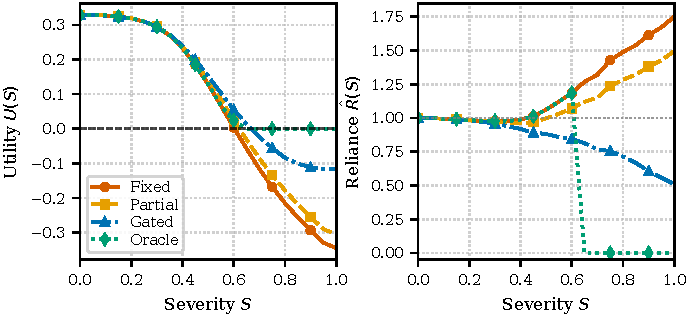
\includegraphics[width=\textwidth]{figures/fig1_synthetic_two_panel.pdf}
\caption{Synthetic benchmark ($N=2000$ test items per seed, 5 seeds, removed null baseline, bootstrap $B=1000$, seed 42). Left: utility $U(S)$ versus severity for Fixed, Partial, Gated, and Oracle models. Right: normalized reliance $\hat R(S)$. The Oracle receives the severity and serves as a positive control; among the other models, Gated has the lowest MI}
\label{fig:synthetic}
\end{figure}

\begin{table}[t]
\centering
\caption{Synthetic benchmark results across architectures and null baselines (Iteration v0.4, $N=2000$ test items per seed, 5 seeds, bootstrap $B=1000$, seed 42).}
\label{tab:synthetic-summary}
\fittable{%
\begin{tabular}{llccccc}
\toprule
\textbf{Model} & \textbf{Null} & \textbf{Clean Acc} & \textbf{Null Acc} & $S^*$ & $\text{MI}_{\text{pooled}}$ & $\text{MI}_{\text{hier}}$ \\
\midrule
Fixed & removed & 0.996 & 0.667 & 0.650 (0.600, 0.650) & 1.491 (1.454, 1.507) & 1.491 (1.373, 1.637) \\
Fixed & zeros & 0.996 & 0.413 & 0.850 (0.850, 0.900) & 0.726 (0.717, 0.741) & 0.726 (0.581, 0.877) \\
Fixed & mean & 0.996 & 0.367 & 0.950 (0.900, 0.950) & 0.862 (0.847, 0.876) & 0.862 (0.670, 1.012) \\
Partial Gated & removed & 0.996 & 0.667 & 0.650 (0.650, 0.650) & 1.286 (1.267, 1.305) & 1.286 (1.196, 1.405) \\
Partial Gated & zeros & 0.996 & 0.416 & 0.900 (0.900, 0.950) & 0.638 (0.629, 0.651) & 0.638 (0.504, 0.781) \\
Partial Gated & mean & 0.996 & 0.377 & 0.950 (0.950, 0.950) & 0.774 (0.766, 0.792) & 0.774 (0.583, 0.927) \\
Gated & removed & 0.996 & 0.667 & 0.700 (0.700, 0.700) & 0.650 (0.639, 0.661) & 0.650 (0.579, 0.752) \\
Gated & zeros & 0.996 & 0.422 & no crossing & no crossing & no crossing \\
Gated & mean & 0.996 & 0.386 & no crossing & no crossing & no crossing \\
Oracle Gated & removed & 0.996 & 0.667 & 0.700 (0.650, 0.700) & 0.000 (0.000, 0.000) & 0.000 (0.000, 0.208) \\
Oracle Gated & zeros & 0.996 & 0.413 & no crossing & no crossing & no crossing \\
Oracle Gated & mean & 0.996 & 0.367 & no crossing & no crossing & no crossing \\
Sharp gate x0.5 & removed & 0.995 & 0.667 & 0.700 (0.650, 0.700) & 0.862 (0.847, 0.876) & 0.862 (0.782, 0.967) \\
Sharp gate x0.5 & zeros & 0.995 & 0.428 & no crossing & no crossing & no crossing \\
Sharp gate x0.5 & mean & 0.995 & 0.401 & no crossing & no crossing & no crossing \\
Sharp gate x1.0 & removed & 0.996 & 0.667 & 0.700 (0.700, 0.700) & 0.650 (0.639, 0.662) & 0.650 (0.580, 0.758) \\
Sharp gate x1.0 & zeros & 0.996 & 0.422 & no crossing & no crossing & no crossing \\
Sharp gate x1.0 & mean & 0.996 & 0.386 & no crossing & no crossing & no crossing \\
Sharp gate x2 & removed & 0.995 & 0.667 & 0.700 (0.700, 0.700) & 0.511 (0.502, 0.522) & 0.511 (0.429, 0.630) \\
Sharp gate x2 & zeros & 0.995 & 0.423 & no crossing & no crossing & no crossing \\
Sharp gate x2 & mean & 0.995 & 0.373 & no crossing & no crossing & no crossing \\
Sharp gate x4 & removed & 0.994 & 0.667 & 0.650 (0.650, 0.700) & 0.470 (0.436, 0.480) & 0.470 (0.360, 0.572) \\
Sharp gate x4 & zeros & 0.994 & 0.444 & no crossing & no crossing & no crossing \\
Sharp gate x4 & mean & 0.994 & 0.368 & no crossing & no crossing & no crossing \\
Sharp gate x8 & removed & 0.992 & 0.667 & 0.650 (0.650, 0.650) & 0.440 (0.430, 0.449) & 0.440 (0.331, 0.545) \\
Sharp gate x8 & zeros & 0.992 & 0.454 & no crossing & no crossing & no crossing \\
Sharp gate x8 & mean & 0.992 & 0.367 & no crossing & no crossing & no crossing \\
Sharp gate x16 & removed & 0.991 & 0.667 & 0.650 (0.650, 0.650) & 0.425 (0.417, 0.434) & 0.425 (0.321, 0.539) \\
Sharp gate x16 & zeros & 0.991 & 0.455 & no crossing & no crossing & no crossing \\
Sharp gate x16 & mean & 0.991 & 0.367 & no crossing & no crossing & no crossing \\
\bottomrule
\end{tabular}}
\end{table}


Table~\ref{tab:synthetic-summary} reports $S^*$ and MI under the removed baseline. The quality-blind Fixed model has the highest MI (\checknum{1.491}{synthetic:FixedModel:MI}), the Partial model \checknum{1.286}{synthetic:PartialGatedModel:MI}, and the Gated model \checknum{0.650}{synthetic:GatedModel:MI}; the Oracle, which receives the severity, reads 0.00. Our first success criterion, a Gated MI below 0.2, was not met: the smooth gate sheds reliance gradually and keeps substantial reliance past the crossing. The pre-declared comparison of independent hierarchical intervals for Fixed and Partial overlapped narrowly ([1.373, 1.637] vs [1.196, 1.405]); a paired bootstrap over seeds and items, added post hoc, supports the ordering $\text{MI}(\text{Gated}) < \text{MI}(\text{Partial}) < \text{MI}(\text{Fixed})$.

% Inlined from sections/results.tex
\section{Evaluation on Vision-Language Models}
\label{sec:results}

\paragraph{Setup.}
We evaluate three open VLMs (Qwen2-VL-2B-Instruct~\cite{wang2024qwen2vl}, LLaVA-1.5-7B in 4-bit~\cite{liu2024improved},
and SmolVLM-Instruct~\cite{marafioti2025smolvlm}) on A-OKVQA multiple-choice questions~\cite{schwenk2022aokvqa}, reading the
next-token distribution over the four option letters. The main sample
contains 500 validation questions; a replication uses disjoint
held-out questions, a new random image-pairing seed, and only the swapped
and Gaussian corruptions. All intervals are 95\% bootstrap intervals over
questions (1000 resamples, fixed seed). The no-input baseline is the
image removed from the prompt unless stated otherwise.

\begin{figure}[tb]
\centering
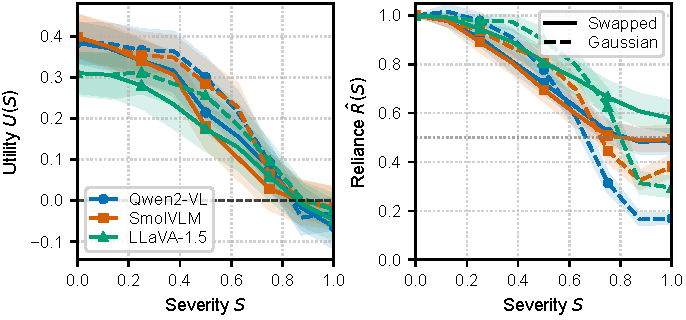
\includegraphics[width=\textwidth]{figures/fig2_vlm_two_panel.pdf}
\caption{Utility (left) and normalized reliance (right) as a function of
  corruption severity for three VLMs under swapped (solid) and Gaussian (dashed)
  corruptions ($N=500$ main sample, removed-image null baseline, bootstrap $B=1000$, seed 42). Shaded bands are 95\% bootstrap intervals}
\label{fig:vlm_curves}
\end{figure}

\paragraph{Residual reliance under a swapped image.}
Table~\ref{tab:headline} reports normalized terminal reliance
$\hat R(1)$ and terminal utility $U(1)$ for each model and corruption.
Across models under the swapped condition, $\hat R(1)$ ranges from
\checknum{0.487}{Qwen:swapblend:R_hat_s1} for Qwen2-VL to
\checknum{0.578}{llava:swapblend:R_hat_s1} for LLaVA-1.5, with SmolVLM at
\checknum{0.493}{SmolVLM:swapblend:R_hat_s1}.
The paired difference in $\hat{R}(1)$ between swapped and Gaussian conditions is
\checknum{+0.32}{paired:Qwen:delta_rhat} (\checknum{0.28}{paired:Qwen:ci_lo}, \checknum{0.37}{paired:Qwen:ci_hi}) for Qwen2-VL,
\checknum{+0.11}{paired:SmolVLM:delta_rhat} (\checknum{0.06}{paired:SmolVLM:ci_lo}, \checknum{0.17}{paired:SmolVLM:ci_hi}) for SmolVLM and
\checknum{+0.28}{paired:llava:delta_rhat} (\checknum{0.23}{paired:llava:ci_lo}, \checknum{0.35}{paired:llava:ci_hi}) for LLaVA-1.5;
every interval excludes zero.
\begin{table}[t]
\centering
\caption{Headline results: terminal normalized reliance $\hat{R}(1)$ and
  terminal utility $U(1)$ for three VLMs under swapped and Gaussian
  corruptions, removed-image null baseline ($B=1000$, seed 42).
  Intervals are 95\% bootstrap CIs.}
\label{tab:headline}
{\footnotesize\setlength{\tabcolsep}{3pt}%
\begin{tabular}{llcc}
\toprule
\textbf{Model} & \textbf{Corruption} & $\hat{R}(1)$ (lo, hi) & $U(1)$ (lo, hi) \\
\midrule
\multicolumn{4}{l}{\textit{Main sample ($N=500$)}} \\
\midrule
Qwen2-VL  & Swapped  & 0.49 (0.44, 0.54) & $-$0.064 ($-$0.114, $-$0.018) \\
          & Gaussian & 0.17 (0.15, 0.19) & $-$0.030 ($-$0.068, $+$0.006) \\
SmolVLM   & Swapped  & 0.49 (0.45, 0.55) & $-$0.016 ($-$0.062, $+$0.030) \\
          & Gaussian & 0.38 (0.34, 0.42) & $-$0.022 ($-$0.068, $+$0.022) \\
LLaVA-1.5 & Swapped  & 0.58 (0.51, 0.65) & $-$0.048 ($-$0.092, $-$0.004) \\
           & Gaussian & 0.30 (0.26, 0.34) & $-$0.022 ($-$0.058, $+$0.014) \\
\midrule
\multicolumn{4}{l}{\textit{Replication ($N=445$)}} \\
\midrule
Qwen2-VL  & Swapped  & 0.47 (0.42, 0.52) & $-$0.103 ($-$0.153, $-$0.052) \\
          & Gaussian & 0.17 (0.14, 0.20) & $-$0.016 ($-$0.058, $+$0.027) \\
SmolVLM   & Swapped  & 0.55 (0.49, 0.62) & $-$0.038 ($-$0.090, $+$0.013) \\
          & Gaussian & 0.32 (0.28, 0.37) & $-$0.029 ($-$0.074, $+$0.013) \\
LLaVA-1.5 & Swapped  & 0.56 (0.50, 0.64) & $-$0.025 ($-$0.072, $+$0.022) \\
           & Gaussian & 0.26 (0.23, 0.30) & $-$0.002 ($-$0.043, $+$0.038) \\
\bottomrule
\end{tabular}}
\end{table}


\paragraph{Utility inversion.}
Terminal utility is significantly below zero under the swapped condition
for Qwen2-VL in both samples, and for LLaVA-1.5 in the main and pooled
samples under the removed-image baseline only; it is not significantly below
zero for SmolVLM. Gaussian corruption does not produce a significant
inversion for any model. Patch masking was also run on the main sample and
produced no significant utility inversion; we omit it for space.
Table~\ref{tab:nullsens} shows how these statements depend on the baseline.

\paragraph{Replication.}
The replication sample in Table~\ref{tab:headline} is consistent with the main result.
Normalized terminal reliance under the swapped condition spans from
\checknum{0.470}{rep:Qwen:swapblend:R_hat_1} for Qwen2-VL to
\checknum{0.563}{rep:llava:swapblend:R_hat_1} for LLaVA-1.5, with SmolVLM at
\checknum{0.553}{rep:SmolVLM:swapblend:R_hat_1}. All three replication
intervals include $0.5$ (lower bound for LLaVA-1.5 is
\checknum{0.497}{rep:llava:swapblend:R_hat_1_ci_lo}).
This replicates the result over questions and pairings, not over models or
datasets.

\paragraph{The pre-declared criterion.}
Before running the main experiment we recorded that a model would show
over-reliance if utility was clearly negative at high severity while
normalized reliance stayed above $0.5$ under the swapped corruption. The
original statement did not specify how ``clearly'' and ``above'' were to
be assessed under sampling uncertainty. We therefore operationalized it
\emph{post hoc} as: the upper bound of the interval for $U(1)$ is below
zero and the lower bound of the interval for $\hat R(1)$ is above $0.5$.
Only \checknum{2}{criterion:status:count_met} of the 42
evaluated combinations satisfy both requirements. Here 42 = model $\times$ corruption $\times$ sample (main, replication, pooled) $\times$ baseline (removed, black); the pooled sample combines main and replication.
The pre-declared criterion is met only for LLaVA-1.5 under the swapped
corruption with the removed baseline, in the main and pooled samples;
none satisfies it in the replication alone or under the black-image baseline.
We treat the pre-declared criterion as largely unsupported and describe
the persistent reliance as a descriptive finding.

\paragraph{Sensitivity to the no-input baseline.}
\label{sec:nullsens}
Table~\ref{tab:nullsens} compares conclusions when the baseline is the
removed image versus a black image. Swapblend reliance changes little for
Qwen2-VL and SmolVLM and falls by about
\checknum{0.084}{nullsens:llava:swapblend:R_hat_drop} for LLaVA-1.5, moving
its interval across $0.5$. Reliance under Gaussian blending drops
substantially under the black null for SmolVLM and LLaVA-1.5 and slightly
for Qwen2-VL. The divergence between the black-image and removed-image
predictions is far larger for SmolVLM and LLaVA-1.5 than for Qwen2-VL; as a
heuristic (since JSD is not additive), the raw unimodal floor accounts for
about \checknum{3.6}{floor:Qwen2-VL-2B-Instruct:fraction_pct}\% of
swapblend $R(1)$ for Qwen2-VL, compared to
\checknum{43}{floor:SmolVLM-Instruct:fraction_pct}\% for SmolVLM and
\checknum{42}{floor:llava-1.5-7b-hf:fraction_pct}\% for LLaVA-1.5. We
hypothesize, without testing it, that this reflects how each model handles
inserted image tokens.
\begin{table}[t]
\centering
\caption{Sensitivity of terminal reliance $\hat{R}(1)$, terminal utility $U(1)$, and unimodal divergence to the choice of null baseline (Removed vs.\ Black image) on the main sample ($N=500$, bootstrap $B=1000$, seed 42). The unimodal floor divergence $\text{JSD}(B_{\text{black}} \parallel B_{\text{removed}})$ is computed over the full sample of all $N=500$ questions (not restricted to the agreement subset) and reported once per model.}
\label{tab:nullsens}
\fittable{%
\begin{tabular}{llccccc}
\toprule
 & & \multicolumn{2}{c}{\textbf{Removed Null Baseline}} & \multicolumn{2}{c}{\textbf{Black Null Baseline}} & \textbf{Full-Sample Unimodal Floor} \\
\cmidrule(lr){3-4} \cmidrule(lr){5-6} \cmidrule(lr){7-7}
\textbf{Model} & \textbf{Corruption} & $U(1)$ & $\hat{R}(1)$ & $U(1)$ & $\hat{R}(1)$ & $\text{JSD}(\text{blk} \parallel \text{rem})$ \\
\midrule
\textbf{Qwen2-VL-2B} & Swapped (Swapblend) & -0.064 (-0.114, -0.018) & 0.487 (0.437, 0.542) & -0.048 (-0.096, -0.002) & 0.468 (0.420, 0.520) & 0.005 (0.004, 0.005) \\
 & Gaussian Blur & -0.030 (-0.068, +0.006) & 0.168 (0.147, 0.189) & -0.014 (-0.052, +0.024) & 0.150 (0.131, 0.170) &  \\
 & Patch Occlusion & -0.006 (-0.030, +0.020) & 0.029 (0.025, 0.033) & +0.010 (-0.012, +0.030) & 0.010 (0.009, 0.012) &  \\
\midrule
\textbf{SmolVLM-Instruct} & Swapped (Swapblend) & -0.016 (-0.062, +0.030) & 0.493 (0.446, 0.547) & -0.002 (-0.046, +0.042) & 0.510 (0.459, 0.568) & 0.077 (0.068, 0.085) \\
 & Gaussian Blur & -0.022 (-0.068, +0.022) & 0.381 (0.337, 0.424) & -0.008 (-0.048, +0.030) & 0.263 (0.231, 0.301) &  \\
 & Patch Occlusion & +0.004 (-0.032, +0.042) & 0.233 (0.206, 0.265) & +0.018 (-0.002, +0.038) & 0.032 (0.026, 0.039) &  \\
\midrule
\textbf{LLaVA-1.5-7B} & Swapped (Swapblend) & -0.048 (-0.092, -0.004) & 0.578 (0.514, 0.653) & -0.040 (-0.082, +0.002) & 0.495 (0.436, 0.563) & 0.069 (0.061, 0.078) \\
 & Gaussian Blur & -0.022 (-0.058, +0.014) & 0.295 (0.255, 0.336) & -0.014 (-0.042, +0.014) & 0.113 (0.091, 0.137) &  \\
 & Patch Occlusion & -0.020 (-0.054, +0.016) & 0.258 (0.224, 0.293) & -0.012 (-0.038, +0.014) & 0.070 (0.057, 0.085) &  \\
\bottomrule
\end{tabular}}
\end{table}


% Inlined from sections/dropout.tex
\section{Case study: modality dropout in a two-view proxy}
\label{sec:fusion}

\paragraph{Setup.}
We train small late-fusion networks on Fashion-MNIST~\cite{xiao2017fashion} split
into left (view A) and right (view B) halves as a two-view proxy. Rather than the
official 10,000-image test split, the 60,000 training images are partitioned
deterministically into 50,000 training, 5,000 validation, and 5,000 test images
(indices 55,000--60,000). View A is degraded toward noise along a nine-point grid,
the null baseline uses a learned embedding, and the gate does not receive the
severity. Models are trained with view-A dropout $p\in\{0,0.1,0.25,0.5\}$ across
five seeds.

\paragraph{Pre-declared hypotheses.}
We declared before training: (H1) the Misalignment Index is non-increasing
in $p$; (H2) clean accuracy falls by less than three points between $p=0$
and $p=0.25$.

\paragraph{Results.}
Table~\ref{tab:fusion} reports the outcome. H2 holds. H1 does \emph{not}:
the Misalignment Index is higher for every $p>0$ than for $p=0$. Between
$p=0$ and $p=0.25$, clean accuracy changes from
\checknum{0.888}{fusion:0.0:clean_acc} to
\checknum{0.884}{fusion:0.25:clean_acc}, a decrease of only
\checknum{0.364}{fusion:diff_0_25:clean_acc_pp} percentage points,
well within the pre-declared three-point bound.
As detailed in Table~\ref{tab:fusion}, dropout-trained models achieve higher
accuracy when view A is removed or degraded, though terminal utility $U(1)$
remains negative across all $p$.
\begin{table}[t]
\centering
\caption{Modality-dropout impact on reliance and accuracy in the
  two-view proxy ($N=5000$ test images, five seeds, learned null
  baseline, $B=1000$). $\hat{R}(1)$ is normalized terminal reliance;
  MI is the Misalignment Index.}
\label{tab:fusion}
{\footnotesize\setlength{\tabcolsep}{3pt}%
\begin{tabular}{ccccccccc}
\toprule
$p$ & Clean Acc & Null Acc & Acc ($S=1$) & $U(1)$ & $R(0)$ & $R(1)$ & $\hat{R}(1)$ & MI \\
\midrule
0.000 & 0.888 & 0.562 & 0.276 & $-$0.286 & 0.331 & 0.611 & 1.846 & 1.657 \\
0.100 & 0.888 & 0.840 & 0.448 & $-$0.392 & 0.056 & 0.452 & 8.105 & 4.586 \\
0.250 & 0.884 & 0.848 & 0.555 & $-$0.293 & 0.040 & 0.330 & 8.362 & 4.514 \\
0.500 & 0.882 & 0.858 & 0.726 & $-$0.133 & 0.024 & 0.148 & 6.200 & 3.684 \\
\bottomrule
\end{tabular}}
\end{table}

\paragraph{Why the normalized measures behave this way (post hoc).}
Reliance at clean input, $R(0)$, falls by more than an order of magnitude as $p$ grows because the model already makes similar predictions with and without view A. Because $\hat{R}$ and MI divide by $R(0)$, they are inflated when $R(0)$ is small, whereas raw reliance $R(1)$ decreases monotonically from \checknum{0.611}{fusion:0.0:R_1_raw} to \checknum{0.148}{fusion:0.5:R_1_raw}.

% Inlined from sections/discussion.tex
\section{Discussion}
\label{sec:discussion}

\paragraph{What the measures reveal.}
We do not claim that VLMs over-trust degraded images in general. The MI is
undefined in most real conditions, so VLM results rest on terminal
reliance and utility, one dataset, and one answer format; the fusion study
is a two-view proxy. The pairing of utility and reliance along a severity
path exposes behaviour that accuracy alone does not: two models can lose the
same accuracy under corruption yet differ in whether that loss comes from
information destruction or persistent reliance on an unhelpful input.
The swapped-image condition consistently produces higher terminal reliance
than Gaussian noise, with gaps whose intervals exclude zero for all three
models, meaning the model's output distribution remains further from its
no-image behaviour when given a wrong image than when given noise.

\paragraph{Baseline sensitivity.}
Conclusions for individual models depend on the no-input baseline. The
black-image and removed-image predictions differ little for Qwen2-VL and
substantially for SmolVLM and LLaVA-1.5: as a heuristic (JSD is not
additive), this divergence equals about
\checknum{3.6}{floor:Qwen2-VL-2B-Instruct:floor_pct}\%,
\checknum{43}{floor:SmolVLM-Instruct:floor_pct}\% and
\checknum{42}{floor:llava-1.5-7b-hf:floor_pct}\% of swapped-image terminal
reliance for the three models. Part of the reliance of SmolVLM and
LLaVA-1.5 may reflect the presence of image tokens and not their content.
Our results suggest that future evaluations report results under at least two
baselines and state how the no-input condition is constructed.

% Inlined from sections/limitations.tex
\section{Limitations}
\label{sec:limitations}

\begin{itemize}
\item \textbf{Null-baseline dependence.} Both utility and reliance are
  defined relative to a no-input baseline; conclusions for individual
  models depend on this choice (see Sect.~\ref{sec:discussion}).

\item \textbf{Multiple comparisons and operationalization after the fact.} The
  pre-declared criterion is evaluated across 42
  model--corruption--sample--baseline combinations without correction; the
  two satisfying combinations overlap (same model, same corruption, different
  sample sizes). The interval-based operationalization of the pre-declared
  criterion was fixed after seeing data; dropout hypotheses H1--H2 were
  committed in the same commit as the training code; the log is not an external
  registry.

\item \textbf{Scope.} One VQA dataset (A-OKVQA, $N=500$ main,
  $N=445$ replication), one multiple-choice format, three models (one in
  4-bit NF4 quantization), one swap pairing per sample. The fusion study
  uses a two-view Fashion-MNIST proxy with simple encoders.

\item \textbf{Prompt sensitivity.} The proportion of probability mass
  assigned to choice letters is sensitive to the prompt template. Models
  whose letter mass falls below 90\% cannot be reliably evaluated under
  our single-token readout.
\end{itemize}

% Inlined from sections/conclusion.tex
\section{Conclusion}
\label{sec:conclusion}

We proposed a severity-indexed diagnostic that pairs utility and
distributional reliance along a degradation path, to separate information
loss from lingering reliance on an input. On synthetic models the measures
order the architectures as intended, although our first success criterion
(Gated MI below 0.2) was not met. On three open VLMs, a swapped-image
corruption leaves normalized reliance at 0.49 to 0.58 of its clean level,
well above Gaussian noise, and produces a significant utility inversion for
one model under both baselines. A criterion declared in advance is met in
only \checknum{2}{criterion:status:count_met} of 42 combinations, and
conclusions for individual models, notably LLaVA-1.5, depend on how the
no-input baseline is defined. The evidence is limited to one dataset, one
answer format and three models. We describe the result as retained
reliance, not over-trust.
Code and per-item outputs will be made available after review.


\bibliographystyle{spmpsci}
\IfFileExists{paper/refs.bib}{%
  \bibliography{paper/refs}%
}{%
  \bibliography{refs}%
}

\end{document}
